\documentclass[12pt,a4paper]{article}

\usepackage[utf8]{inputenc}
\usepackage{geometry}
\usepackage{indentfirst}
\usepackage{graphicx}

\geometry{margin=2.5cm}
\setlength{\parindent}{1.25cm}
\linespread{1.3}

\title{\textbf{Manual de Instalação e Operação}\\Agentic Customer Intelligence}
\author{Gabriel Cravalho Domingos da Conceição}
\date{Maio de 2026}

\begin{document}

\maketitle

\section{Objetivo}

Este manual descreve os componentes necessários para instalar, configurar e executar localmente o ambiente do projeto Agentic Customer Intelligence. O projeto contém pipeline de clusterização, backend RAG de personas, persistência em banco de dados, interface web e integração com uma API local compatível com OpenAI.

\section{Pré-requisitos}

\begin{itemize}
  \item Linux ou ambiente compatível com shell Bash.
  \item Python 3.11 ou superior.
  \item \texttt{uv} instalado.
  \item Docker e Docker Compose.
  \item Node.js 20 ou superior.
  \item npm.
  \item API local compatível com OpenAI para chat e embeddings.
  \item Opcional: Jupyter Notebook ou JupyterLab para executar o notebook de ML.
\end{itemize}

\section{Estrutura Principal do Projeto}

\begin{verbatim}
agentic-customer-intelligence/
|-- data/
|-- ml-clustering/
|-- agentic-personas/
|   |-- backend/
|   |-- knowledge_base/
|   `-- src/
|-- apps/web/
|-- infra/
|-- docs/
|-- docker-compose.yml
|-- pyproject.toml
`-- uv.lock
\end{verbatim}

\section{Componentes do Ambiente}

\begin{itemize}
  \item \textbf{PostgreSQL + pgvector}: armazena embeddings e chunks da base de conhecimento.
  \item \textbf{MongoDB}: armazena conversas e histórico de mensagens.
  \item \textbf{Backend FastAPI 8010}: API principal das personas e do chat RAG.
  \item \textbf{Frontend React 5173}: interface web para chat coletivo e individual.
  \item \textbf{API agentic 8020}: API auxiliar do pacote \texttt{agentic\_personas}.
  \item \textbf{LLM local 8000}: serviço compatível com OpenAI, usado para chat e embeddings.
\end{itemize}

\section{Configuração Inicial}

\subsection{Instalar dependências Python}

Na raiz do projeto:

\begin{verbatim}
uv sync
\end{verbatim}

\subsection{Configurar variáveis de ambiente}

Copie os arquivos de exemplo:

\begin{verbatim}
cp .env.example .env
cp agentic-personas/backend/.env.example agentic-personas/backend/.env
cp apps/web/.env.example apps/web/.env
\end{verbatim}

Principais variáveis:

\begin{verbatim}
OPENAI_BASE_URL=http://127.0.0.1:8000/v1
OPENAI_API_KEY=local
OPENAI_MODEL=qwen-linkedin
OPENAI_EMBEDDING_MODEL=embed-local
EMBEDDING_DIM=768

POSTGRES_HOST=localhost
POSTGRES_PORT=5432
POSTGRES_DB=agentic_customer_intelligence
POSTGRES_USER=aci
POSTGRES_PASSWORD=aci

MONGO_HOST=localhost
MONGO_PORT=27017
MONGO_DB=agentic_customer_intelligence
MONGO_COLLECTION=conversations

VITE_API_BASE_URL=http://127.0.0.1:8010/api
\end{verbatim}

Observação: \texttt{EMBEDDING\_DIM} deve ser compatível com a dimensão retornada pelo serviço local de embeddings.

\section{Subir Bancos de Dados}

Na raiz do projeto:

\begin{verbatim}
docker-compose up -d mongo postgres
\end{verbatim}

Verificação:

\begin{verbatim}
docker ps
\end{verbatim}

Serviços esperados:

\begin{itemize}
  \item \texttt{aci-mongo} em \texttt{localhost:27017};
  \item \texttt{aci-postgres} em \texttt{localhost:5432}.
\end{itemize}

\section{Subir a API Local de LLM}

O backend espera um serviço compatível com OpenAI, expondo:

\begin{verbatim}
POST /v1/chat/completions
POST /v1/embeddings
\end{verbatim}

Exemplo de verificação:

\begin{verbatim}
curl http://127.0.0.1:8000/v1/models \
  -H "Authorization: Bearer local"
\end{verbatim}

Este projeto não fixa uma implementação única do LLM. Pode-se usar uma API local baseada em llama.cpp, vLLM, Ollama com proxy compatível, ou outro servidor que respeite o formato OpenAI.

\section{Executar Pipeline de Machine Learning}

Para regenerar perfis de cluster:

\begin{verbatim}
PYTHONPATH=ml-clustering/src \
uv run python ml-clustering/run_pipeline.py
\end{verbatim}

Para gerar resumo executivo da parte de ML:

\begin{verbatim}
PYTHONPATH=ml-clustering/src \
uv run python ml-clustering/generate_part1_summary.py
\end{verbatim}

Para abrir o notebook Jupyter:

\begin{verbatim}
uv run jupyter notebook \
  ml-clustering/notebooks/customer_segmentation_clustering.ipynb
\end{verbatim}

Os principais outputs são escritos em:

\begin{verbatim}
ml-clustering/outputs/
\end{verbatim}

\section{Ingerir Base de Conhecimento RAG}

Com PostgreSQL, pgvector e API de embeddings ativos:

\begin{verbatim}
PYTHONPATH=agentic-personas/backend \
uv run python agentic-personas/backend/scripts/ingest_knowledge_base.py
\end{verbatim}

Esse script recria a tabela vetorial:

\begin{verbatim}
persona_knowledge_chunks
\end{verbatim}

\section{Subir Backend Principal}

Na raiz do projeto:

\begin{verbatim}
cd agentic-personas/backend
PYTHONPATH=/caminho/para/agentic-customer-intelligence/agentic-personas/backend \
uv run uvicorn app.main:app --host 0.0.0.0 --port 8010 --reload
\end{verbatim}

Substitua \texttt{/caminho/para/...} pelo caminho local do projeto.

Verificação:

\begin{verbatim}
curl http://127.0.0.1:8010/api/health
\end{verbatim}

Resposta esperada:

\begin{verbatim}
{"status":"ok","app_name":"Agentic Customer Intelligence API"}
\end{verbatim}

\section{Subir Frontend}

Instale dependências na primeira execução:

\begin{verbatim}
cd apps/web
npm install
\end{verbatim}

Execute o servidor Vite:

\begin{verbatim}
npm run dev -- --host 0.0.0.0 --port 5173 --strictPort
\end{verbatim}

Acesse:

\begin{verbatim}
http://localhost:5173
\end{verbatim}

O uso de \texttt{--strictPort} é recomendado para evitar que o Vite suba silenciosamente em outra porta caso a porta 5173 esteja ocupada.

\section{Subir API Agentic Auxiliar}

Na raiz do projeto:

\begin{verbatim}
PYTHONPATH=/caminho/para/agentic-customer-intelligence/agentic-personas/src \
uv run uvicorn agentic_personas.api:app --host 0.0.0.0 --port 8020 --reload
\end{verbatim}

Esse componente é auxiliar e pode ser usado para exploração do pacote \texttt{agentic\_personas}.

\section{Comando Integrado de Desenvolvimento}

Um fluxo típico de desenvolvimento envolve três terminais:

\begin{enumerate}
  \item bancos e LLM local;
  \item backend principal na porta 8010;
  \item frontend na porta 5173.
\end{enumerate}

Exemplo:

\begin{verbatim}
docker-compose up -d mongo postgres

cd agentic-personas/backend
PYTHONPATH=$(pwd) uv run uvicorn app.main:app \
  --host 0.0.0.0 --port 8010 --reload

cd ../../apps/web
npm run dev -- --host 0.0.0.0 --port 5173 --strictPort
\end{verbatim}

\section{Guia Prático de Uso da Ferramenta}

Após subir os serviços, abra \texttt{http://localhost:5173}. O fluxo prático de uso é:

\begin{enumerate}
  \item Criar uma conversa com o botão \texttt{Nova conversa}.
  \item Escolher \texttt{Chat coletivo com as 3 personas} para comparação simultânea.
  \item Ou clicar em \texttt{Conversar com esta persona} em um card para chat individual.
  \item Digitar a pergunta no campo inferior e enviar no botão de envio.
\end{enumerate}

Botões e ações principais na interface:

\begin{itemize}
  \item \texttt{Nova conversa}: cria um novo contexto de chat.
  \item \texttt{Limpar tudo}: remove o histórico local de conversas da barra lateral.
  \item \texttt{Regenerate}: gera novamente a última resposta com o mesmo prompt.
  \item \texttt{Edit + Resend}: permite editar a pergunta e reenviar.
  \item \texttt{Limpar}: limpa mensagens da conversa atual.
  \item \texttt{Excluir}: remove a conversa atual.
\end{itemize}

Guia rápido para usar melhor:

\begin{itemize}
  \item Perguntas de comparação: use chat coletivo.
  \item Perguntas táticas por segmento: use chat individual.
  \item Perguntas de preço e promoção: peça contraste explícito entre as três personas.
  \item Para sessões de demo: inicie por uma pergunta ampla e depois aprofunde por persona.
\end{itemize}

\section{Menu Run and Debug (VS Code)}

Se o workspace estiver com as configurações de execução carregadas, o menu \textit{Run and Debug} expõe atalhos para subir e parar os serviços sem usar terminal manualmente.

\begin{figure}[htbp]
\centering
\IfFileExists{run_and_debug_menu.png}{
  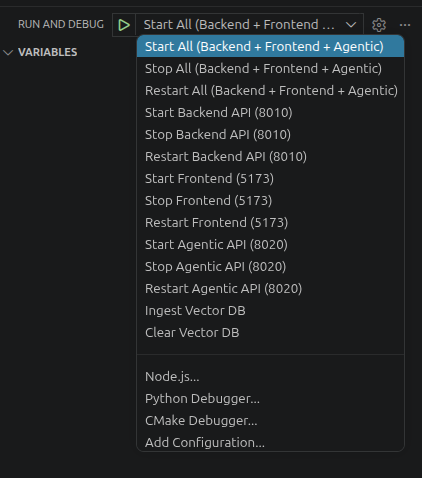
\includegraphics[width=0.55\textwidth]{run_and_debug_menu.png}
}{
  \fbox{\parbox{0.85\textwidth}{
  Arquivo de screenshot nao encontrado.\\
  Adicione a imagem em: \texttt{docs/run\_and\_debug\_menu.png}
  }}
}
\caption{Menu Run and Debug com atalhos de orquestracao local}
\end{figure}

\subsection{Atalhos combinados}

\begin{itemize}
  \item \texttt{Start All (Backend + Frontend + Agentic)}: inicia backend 8010, frontend 5173 e API agentic 8020.
  \item \texttt{Stop All (Backend + Frontend + Agentic)}: encerra os três serviços.
  \item \texttt{Restart All (Backend + Frontend + Agentic)}: reinicia os três serviços.
\end{itemize}

\subsection{Atalhos por serviço}

\begin{itemize}
  \item \texttt{Start Backend API (8010)} / \texttt{Stop Backend API (8010)} / \texttt{Restart Backend API (8010)}.
  \item \texttt{Start Frontend (5173)} / \texttt{Stop Frontend (5173)} / \texttt{Restart Frontend (5173)}.
  \item \texttt{Start Agentic API (8020)} / \texttt{Stop Agentic API (8020)} / \texttt{Restart Agentic API (8020)}.
\end{itemize}

\subsection{Ações de base vetorial}

\begin{itemize}
  \item \texttt{Ingest Vector DB}: executa ingestão dos arquivos da base de conhecimento no PostgreSQL/pgvector.
  \item \texttt{Clear Vector DB}: limpa os dados vetoriais previamente ingeridos.
\end{itemize}

\subsection{Fluxo recomendado com os botões}

\begin{enumerate}
  \item Executar \texttt{Start All (Backend + Frontend + Agentic)}.
  \item Executar \texttt{Ingest Vector DB} ao atualizar conteúdos em \texttt{knowledge\_base}.
  \item Abrir \texttt{http://localhost:5173} e validar a tela inicial.
  \item Ao finalizar, executar \texttt{Stop All (Backend + Frontend + Agentic)}.
\end{enumerate}

\section{Endpoints Úteis}

\begin{itemize}
  \item \texttt{GET /api/health}: status da API.
  \item \texttt{GET /api/personas}: lista personas.
  \item \texttt{GET /api/personas/\{cluster\_id\}}: detalhe de persona.
  \item \texttt{POST /api/chat}: chat não-streaming.
  \item \texttt{POST /api/chat/stream}: chat streaming.
  \item \texttt{POST /api/retrieval/test}: teste de recuperação RAG.
  \item \texttt{POST /api/conversations}: cria conversa.
  \item \texttt{GET /api/conversations}: lista conversas.
  \item \texttt{PATCH /api/conversations/\{id\}}: atualiza título.
  \item \texttt{DELETE /api/conversations/\{id\}}: exclui conversa.
  \item \texttt{DELETE /api/conversations/\{id\}/messages}: limpa mensagens.
\end{itemize}

\section{Validação de Qualidade}

Para executar a bateria de avaliação das respostas:

\begin{verbatim}
uv run python agentic-personas/backend/scripts/evaluate_persona_quality.py
\end{verbatim}

Arquivos gerados:

\begin{verbatim}
agentic-personas/backend/outputs/persona_answer_battery.json
docs/persona_answer_battery_report.md
\end{verbatim}

\section{Build de Produção do Frontend}

\begin{verbatim}
cd apps/web
npm run build
\end{verbatim}

O resultado é gerado em:

\begin{verbatim}
apps/web/dist/
\end{verbatim}

Esse diretório é artefato de build e não deve ser versionado.

\section{Limpeza e Solução de Problemas}

\subsection{Porta do Vite ocupada}

Listar processos:

\begin{verbatim}
lsof -iTCP:5173 -sTCP:LISTEN -n -P
\end{verbatim}

Encerrar processo:

\begin{verbatim}
kill <PID>
\end{verbatim}

\subsection{Backend não responde}

Verificar portas:

\begin{verbatim}
lsof -iTCP:8010 -sTCP:LISTEN -n -P
\end{verbatim}

Verificar health:

\begin{verbatim}
curl http://127.0.0.1:8010/api/health
\end{verbatim}

\subsection{Erro de embeddings}

Verifique:

\begin{itemize}
  \item se a API local de LLM está ativa;
  \item se \texttt{OPENAI\_BASE\_URL} está correto;
  \item se \texttt{OPENAI\_EMBEDDING\_MODEL} existe no servidor local;
  \item se \texttt{EMBEDDING\_DIM} corresponde ao vetor retornado.
\end{itemize}

\subsection{Recriar bancos}

Atenção: o comando abaixo remove volumes persistidos.

\begin{verbatim}
docker-compose down -v
docker-compose up -d mongo postgres
\end{verbatim}

\section{Ordem Recomendada para Demo}

\begin{enumerate}
  \item Subir MongoDB e PostgreSQL.
  \item Subir API local de LLM e embeddings.
  \item Rodar ingestão da base de conhecimento.
  \item Subir backend principal em \texttt{8010}.
  \item Subir frontend em \texttt{5173}.
  \item Abrir \texttt{http://localhost:5173}.
  \item Usar chat coletivo ou cards de personas individuais.
\end{enumerate}

\end{document}
